\documentclass{article}

%............Inicia Preambulo.......................
\usepackage{graphicx}
\usepackage{float}
\usepackage[utf8]{inputenc}
\usepackage[shortlabels]{enumitem}
\usepackage{textcomp}
\usepackage{multicol}
\usepackage{caption}
\usepackage[spanish]{babel}
\usepackage[total={17.5cm, 23cm}, top=2cm, left=2cm]{geometry}
\usepackage{esvect}
\usepackage[font=footnotesize]{caption}

\spanishdecimal{.}
\parindent 0cm

%.............Fin de Preambulo........................

\begin{document}

\begin{center}
{\Large \textbf{Universidad Autónoma de Coahuila}}
\end{center}

\begin{center}
{\large Facultad de Ciencias Físico-Matemáticas}
\end{center}

%Materia
\begin{center}
{\large Metodos Numericos}
\end{center}

%Título
\begin{center}
{\large Interpolacion por Lagrange}
\end{center}

%Fecha
\begin{center}
{\large 02 de Diciembre del 2019}
\end{center}

%Autor
\begin{center}
{\large José Antonio Olveda García}
\end{center}

\vspace{5mm}

\begin{multicols}{2}

\section{Objetivo}
\label{sec:obj}
  Analizar el como el metodo de interpolacion es mas preciso que el metodo de interpolacion simple, ajustando una serie de datos para poder encontrar nuestro polinomio de solucion

\section{Introduccion}
\label{sec:Intro}
\textbf{¿Que es la interpolacion?}
\\
La interpolacion consiste en hallar un dato dentro de un intervalo en el que conocemos los valores de los extremos
\\

\textbf{¿Que es la Interpolacion Polinomica?}
\\
El objetivo es hallar un polinomio que pase por los puntos y permita hallar aproximaciones de otros valores desconocidos para la funcion.

\section{Metodología Experimental}
\label{sec:Met}
\textbf{Interpolacion por Lagrange}
\\
Se trata de construir un polinomio de grado n, que se anule en los puntos (que pase por los puntos): 
$(x_{0},y_{0}), (x_{1},y_{1}),... ,(x_{n},y_{n})$ salvo en uno $(x_{j})$  en el que valdra 1.
Dicho polinomio será de la forma:
\begin{equation}
P_{n}(x)=a \prod_{i=0}^{n} \frac{x-x_{i}}{x_{k}-x_{i}} =$$
\\
$$ \frac{x-x_{0}...(x-x_{k-1})(x-x_{k+1})...(x-x_{n})}{(x_{k}-x_{0})...(x_{k}-x_{k-1})(x_{k}-x_{k+1})...(x_{k}-x_{n})}
\end{equation}

y para que el polinomio interpolador de grado n, que buscamos, tome los valores $y_{0}$, $y_{1}$, ... , $y_{n}$ en los puntos $x_{0}$,$x_{1}$, ... , $x_{n}$, es suficiente con que se verifique:
\begin{equation}
P_{n}(x)= \sum_{k=0}^{n} f(x_{k})l_{k}(x)
\end{equation}

llamándose dicha expresión fórmula de Lagrange del polinomio de interpolación y a los lk polinomios de Lagrange.

\section{Ejemplo}
\label{sec:Ejem}
Construir el polinomio interpolador por el método de Lagrange, que pase por los puntos:

\begin{center}
$(1,1.5), (2,3.9), (3,9), (4,15)$
\end{center}

siendo el polinomio interpolador: 

\begin{center}
$$P_{n}(x)= \sum_{k=0}^{n} f(x_{k})l_{k}(x)$$
\end{center}

Así mismo:

\begin{center}
$$P_{n}(x)=a \prod_{i=0}^{n} \frac{x-x_{i}}{x_{k}-x_{i}} $$
\end{center}

y 
\begin{center}
$$ l_{n}(x_{n})= \frac{(x_{n}-x_{0})(x_{n}-x_{1})...(x_{n}-x_{n-1})}{(x_{n}-x_{0})(x_{n}-x_{1})(x_{n}-x_{n+1})}=1$$
\end{center}

por tanto

\begin{center}
$P_{n}(x)=f(x_{n})$
\end{center}

Por ello, introduciendo los datos, se obtienen finalmente el polinomio interpolador el cual es:

\begin{center}
$$P_{3}(x)=0.3x^{3}+3.15x^{2}-4.95x+3.6$$
\end{center}
\section{Ventajas y Desventajas}
\label{sec:Ven}
\textbf{Ventajas}
\\
1. Se puede aplicar si la tabla no esta igualmente espaciada.
\\
2. Se puede aplicar en toda la tabla.
\\
3. No requiere tabla de diferencias.
\\
4. Es fácil de programar.
\\
\\
\textbf{Desventajas}
\\
1. No da el grado del polinomio.
\\
2. Es complicado para cálculos manuales.
\\
3. Cuando el numero de datos tiene que aumentar o disminuir, no se pueden utilizar los resultados de los calculos previos.
\\
4. La evaluacion del error no es facil.
\section{Implementacion del programa}
\label{sec:Imp}
\begin{figure}[H]
\centering
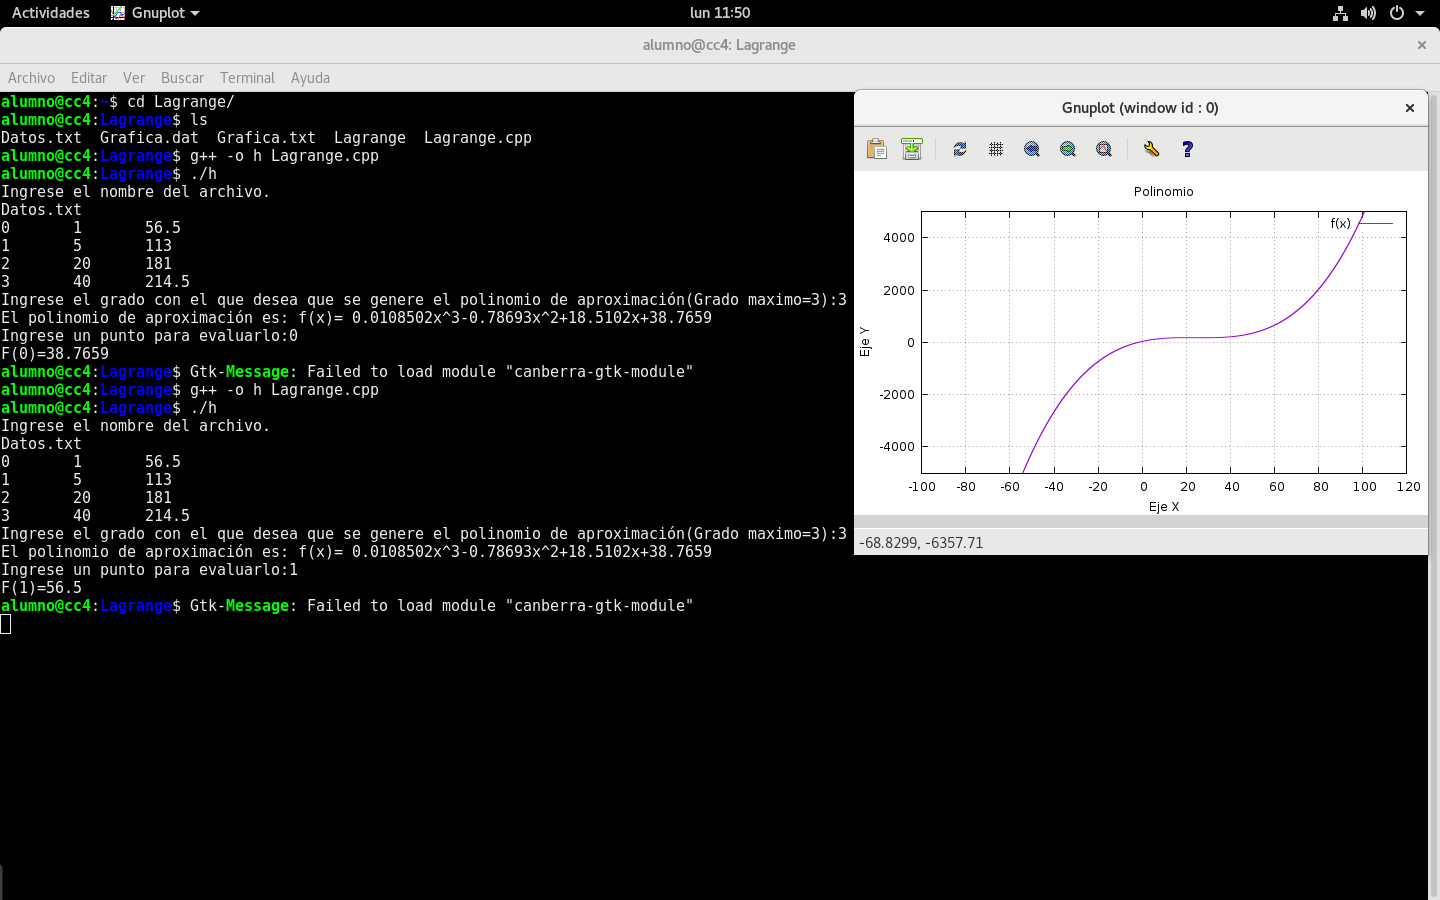
\includegraphics[scale=.125]{Lagrange.png}
\caption{Aplicacion del programa de lagrange}
\end{figure}
Como podemos ver en la figura mostrada, se puede aplicar los datos de un ejercicio aplicado en clase, donde se gernera algo similar al productorio a partir del programa aplicado, para facilitar la ingresion de datos, se pide al igual que el programa de interpolacion un archivo de datos.txt para evitar ingresar dichos datos.


\end{multicols}

\end{document}
